%---------------------导言区---------------------------%
\documentclass[12pt,a4paper,UTF8]{ctexart}
	%10pt:正文字体为12pt,缺省为10pt;各层级字体大小会根据正文字体自动调整
	%a4paper:纸张大小a4;
	%UTF8:中文要求
\CTEXsetup[format={\Large\bfseries}]{section}
\usepackage{geometry}%用于设置上下左右页边距
\usepackage{makecell}
	\geometry{left=2.5cm,right=2.5cm,top=3.2cm,bottom=2.8cm}
\usepackage{xeCJK,amsmath,paralist,enumerate,booktabs,multirow,graphicx,subfig,setspace,listings,lastpage,hyperref}
	%xeCJK:中文字体(如楷体,作者和机构需要用到)的设置
	%amsmath:数学公式
	%paralist,enumerate:自定义项目符号
	%booktabs:三线图,论文常用的表格风格
	%multirow:复杂表格
	%graphicx,float: 插入图片
	%subfig:并排排版图片、竖向排版图片
	%setspace:设置行间距等功能
	\setlength{\parindent}{2em}%正文首行缩进两个汉字
	%listings:用于排版各种代码;比如matlab的代码
	\lstset{language=Matlab}%matlab代码
	%lastpage:获取总页数;
	%hyperref:超链接,和lastpage搭配.
\usepackage{fancyhdr}
	%fancyhdr:一个很强大的宏包,用于自定义设计页面风格并命名以供调用。
	\pagestyle{fancy}
	\rhead{实验C1 电子电荷的确定——密立根油滴实验}
	\lhead{基础物理实验\uppercase\expandafter{\romannumeral2}实验报告}
	\cfoot{Page \thepage/\pageref{LastPage}}  %当前页\总页数
	\rfoot{\today}
		%分别是右页眉、左页眉、中页脚、右页脚
	\renewcommand{\headrulewidth}{0.4pt}
	\renewcommand{\theenumi}{(\arabic{enumi})}

% \setCJKmainfont{FZShuSong-Z01S}[ItalicFont=FZKai-Z03S, BoldFont=FZHei-B01S]
%中文字体设置:使用开源字体方正书宋,方正楷体和方正黑体



%%%%%%%%%%%%%%%%%%%%%%%%%%%%%%%%%%%%%%%%%%%%%%%%%%%%%%%%%%
%%%%%%%%%%%%%%%%%%%%%%%%%正文开始%%%%%%%%%%%%%%%%%%%%%%%%%%
%%%%%%%%%%%%%%%%%%%%%%%%%%%%%%%%%%%%%%%%%%%%%%%%%%%%%%%%%%

\begin{document}

%%begin-------------------标题与信息-----------------------%%

%%标题
\begin{center}
\LARGE\textbf{实验C1 电子电荷的确定——密立根油滴实验}
\end{center}

%%end-------------------标题与信息-----------------------%%


\section*{【数据处理与分析】}
\begin{table}[htbp]
	\caption{密立根油滴实验参数}
	\centering
    \begin{tabular}{ccc|ccc}
	\toprule
	符号 & 物理意义 & 数值和单位 & 符号 & 物理意义 & 数值和单位  \\
	\midrule
	d & 极板间距 & $5.00 \times 10^{-3}m$ & g & 重力加速度 & $9.78858 m/s^2$\\
	$\eta$ & 空气黏滞系数 & $1.83 \times 10^{-5}kg/(m \cdot s)$ & $\rho$ & 油的密度 & $981 kg/m^3 (20 ^{\circ}C)$\\
    b & 修正常数 & $6.17 \times 10^{-6}m/cmHg$ & p & 大气压强 & 76.0mmHg \\
    l & 下落距离 & 1.6mm & V & 平衡电压 & \\
    $t_g$ & 油滴下落时间 & & $t_e$ & 油滴上升时间 & \\
	\bottomrule
    \end{tabular}%注意这里还有一个半括号
\label{tab:1}%
\end{table}

\subsection*{1.	静态(平衡)测量法}
由油滴在极板间受力平衡及斯托克斯公式可得油滴半径为:
\begin{equation}\label{eq:1}
    a=\left[\frac{9\eta l}{2\rho g t_g}\right]^{1/2} 
\end{equation}

进而求出带电量q:
\begin{equation}\label{eq:2}
    q=\frac{18\pi}{\sqrt{2\rho g}}\left[\frac{\eta l}{t_g \left(1+\frac{b}{pa}\right) }\right]^{3/2} \frac{d}{V} 
\end{equation}

将实验数据代入公式\ref{eq:1}和公式\ref*{eq:2}得到结果见表\ref*{tab:2}:

\begin{table}[!h]
	\centering
	\caption{静态测量法计算结果}	  
	\begin{tabular}{c|ccccccc}
	\toprule
	\multicolumn{1}{c}{} & 实验次数  & 1  & 2   & 3 & 4 & 5 &平均值  \\
	\midrule
	\multicolumn{1}{c}{\multirow{2}[2]{*}{油滴1}} & 油滴半径$a/10^{-7}m$     & 10.77 & 10.74  & 10.60 & 10.62 & 10.59& 10.66\\
	\multicolumn{1}{c}{} & 电荷$q/10^{-19}C$     & 21.84 & 21.91  & 20.79 & 20.53 &20.57& 21.13 \\
	\midrule
	\multicolumn{1}{c}{\multirow{2}[2]{*}{油滴2}} & 油滴半径$a/10^{-7}m$     & 6.91 & 7.16  & 7.06 & 7.02 & 6.99 & 7.03\\
	\multicolumn{1}{c}{} & 电荷$q/10^{-19}C$    & 4.46 & 4.95  & 4.70 & 4.65 & 4.54 & 4.54 \\
    \midrule
	\multicolumn{1}{c}{\multirow{2}[2]{*}{油滴3}} & 油滴半径$a/10^{-7}m$      & 9.37 & 9.43  & 9.47 & 9.31 & 9.35 & 9.39\\
	\multicolumn{1}{c}{} & 电荷$q/10^{-19}C$     & 9.62 & 9.75  & 9.75 & 9.50 & 9.49 & 9.49\\
	\midrule
	\multicolumn{1}{c}{\multirow{2}[2]{*}{油滴4}} & 油滴半径$a/10^{-7}m$      & 8.33 & 8.52 & 8.23 & 8.49 & 8.50 & 8.41\\
	\multicolumn{1}{c}{} & 电荷$q/10^{-19}C$     & 9.44 & 9.95 & 8.70 & 10.03 & 9.96 & 9.96 \\
    \midrule
    \multicolumn{1}{c}{\multirow{2}[2]{*}{油滴5}} & 油滴半径$a/10^{-7}m$      & 8.75 & 8.85  & 8.78 & 8.96 & 8.86 & 8.84\\
	\multicolumn{1}{c}{} & 电荷$q/10^{-19}C$     & 8.06 & 8.05  & 7.939 & 8.63 & 8.13 & 8.13 \\
	\bottomrule
	\end{tabular}%
    \label{tab:2}
\end{table}%

为证明电荷的不连续性和所有电量都是基本电荷 e 的整数倍,并得到基本电荷 e 值(即电子的电荷量),需对实验测得的各个电量 q 求最大公约数。
若测量误差较大,求出 q 的最大公约数比较困难,通常需采用“倒过来验证”的办法进行数据处理。用实验测得的电量 q 除以公认的电子电荷值 $e =1.602177\times 10^{-19}C$,可得一个接近整数的数值,这个整数就是油滴所带的基本电荷的数目 n 。
再用这个 n 去除实验测得的电量,就得到电子的电荷值 e 。

计算数据见表\ref*{tab:3}:

\begin{table}[!h]
	\centering
	\caption{静态法油滴带电量及所带元电荷数目}	  
	\begin{tabular}{ccccc}
	\toprule
	油滴编号 & \makecell[c]{油滴所带电荷量\\$q/10^{-19}C$} & 元电荷数目n & \makecell[c]{测得电子电荷值\\$q/10^{-19}C$} & 相对误差\\
	\midrule
	1 & 21.13 & 13 & 1.63 & 1.88 \\
	2 & 4.54 & 3 & 1.51 & 0.56 \\
	3 & 9.49 & 6 & 1.58 & 1.25 \\
	4 & 9.96 & 6 & 1.66 & 3.75 \\
	5 & 8.13 & 5 & 1.63 & 1.86 \\
	\bottomrule
\end{tabular}%
\label{tab:3}
\end{table}%

以 q 为纵坐标,n 为横坐标做散点图,并用y = ax曲线拟合,拟合结果斜率为元电荷 e 的测量值,即 e=a。根据最小二乘法拟合直线得图\ref*{fig:1}:

\begin{figure}[!h]
	\centering
	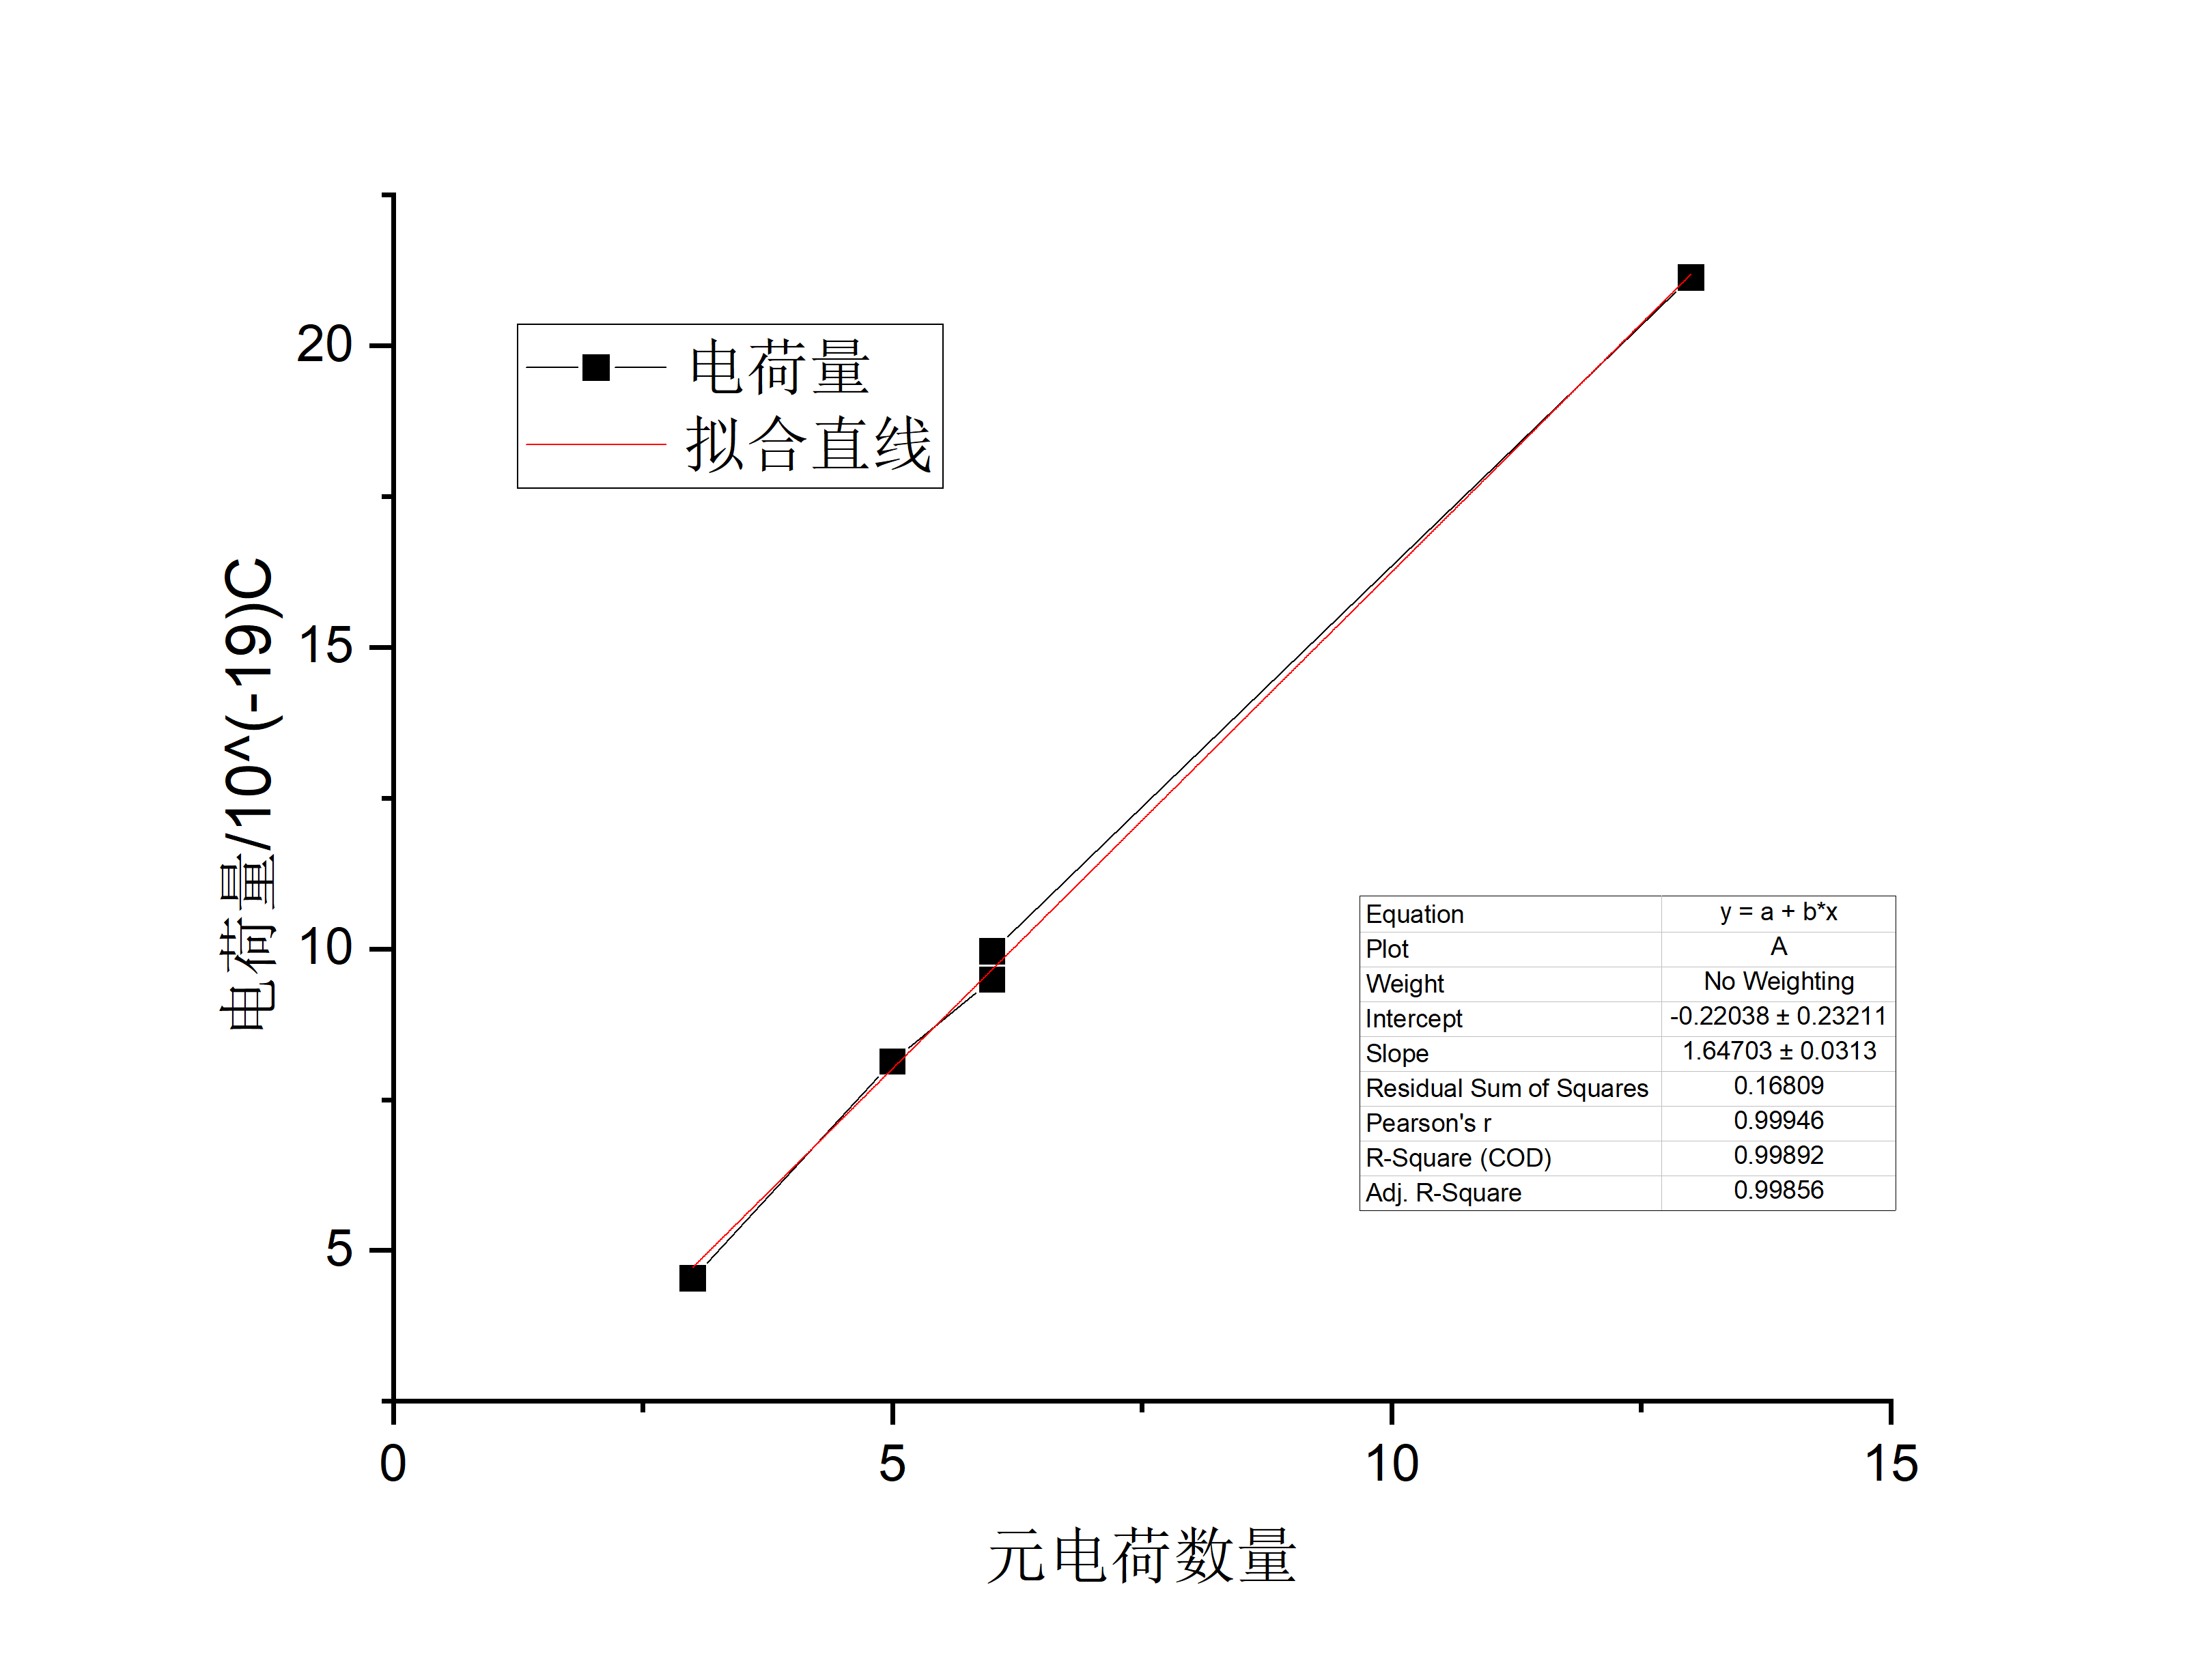
\includegraphics[width=0.6\textwidth]{img//1.png}
		%textwidth:正文宽度。双栏,则将两栏正文宽度相加。
	\caption{静态测量法的q-n拟合曲线}
	\label{fig:1}
\end{figure}

通过静态测量法实验测得的元电荷的平均值为$1.64703 \times 10^{-19}C$,与标准值$e =1.602177\times 10^{-19}C$相对误差为2.80\%.

\subsubsection*{误差分析}

静态法产生误差的原因可能有:

\begin{enumerate}
	\item 锁定的平衡电压不够准确
	\item 计时时人为反应与机器显示延时导致测量下落时间有误差
	\item 实验当时空气湿度极端导致空气粘滞指数与给定值不一致
	\item 实验当天温度对应的油滴密度与给定值不同
\end{enumerate}

\subsection*{2.	动态(非平衡)测量法}

由公式\ref*{eq:3}可以计算油滴电荷量:

\begin{equation}\label{eq:3}
    q=\frac{18\pi}{\sqrt{2\rho g}}\left[\frac{\eta l}{\left(1+\frac{b}{pa}\right) }\right]^{3/2} \frac{d}{V} \left(\frac{1}{t_e}+\frac{1}{t_g}\right) \left(\frac{1}{t_g}\right)^{1/2}  
\end{equation}

将实验数据代入公式\ref{eq:1}和公式\ref*{eq:3}得到结果见表\ref*{tab:4}:

\begin{table}[!h]
	\centering
	\caption{动态测量法计算结果}	  
	\begin{tabular}{c|ccccccc}
	\toprule
	\multicolumn{1}{c}{} & 实验次数  & 1  & 2   & 3 & 4 & 5 &平均值  \\
	\midrule
	\multicolumn{1}{c}{\multirow{2}[2]{*}{油滴1}} & 油滴半径$a/10^{-7}m$     & 9.36 & 9.42 & 9.32 & 9.28 & 9.25 & 9.32\\
	\multicolumn{1}{c}{} & 电荷$q/10^{-19}C$     & 8.16 & 8.26 & 8.24 & 8.00 & 7.88 & 8.11\\
	\midrule
	\multicolumn{1}{c}{\multirow{2}[2]{*}{油滴2}} & 油滴半径$a/10^{-7}m$     & 8.85 & 8.72 & 8.78 & 8.80 & 8.92 & 8.81\\
	\multicolumn{1}{c}{} & 电荷$q/10^{-19}C$    & 9.35 & 9.06  & 9.17 & 9.29 & 9.42 & 9.26\\
    \midrule
	\multicolumn{1}{c}{\multirow{2}[2]{*}{油滴3}} & 油滴半径$a/10^{-7}m$      & 11.88 & 12.00 & 11.85 & 11.99 & 11.94 & 11.93\\
	\multicolumn{1}{c}{} & 电荷$q/10^{-19}C$     & 27.37 & 28.36 & 27.92 & 28.34 & 28.04 & 28.01\\
	\midrule
	\multicolumn{1}{c}{\multirow{2}[2]{*}{油滴4}} & 油滴半径$a/10^{-7}m$      & 9.10 & 9.03 & 9.20 & 9.09 & 9.20 & 9.13\\
	\multicolumn{1}{c}{} & 电荷$q/10^{-19}C$     & 14.39 & 14.12  & 14.17 & 14.04 & 14.20 & 14.18\\
    \midrule
    \multicolumn{1}{c}{\multirow{2}[2]{*}{油滴5}} & 油滴半径$a/10^{-7}m$      & 11.33 & 11.02 & 11.30 & 11.44 & 11.17 & 11.25\\
	\multicolumn{1}{c}{} & 电荷$q/10^{-19}C$     & 26.78 & 25.11 & 27.85 & 27.62 & 25.65 & 26.60\\
	\bottomrule
	\end{tabular}%
    \label{tab:4}
\end{table}%

用同样方法计算得电量 q 、基本电荷的数目 n 及元电荷电量 e。

\begin{table}[!h]
	\centering
	\caption{动态法油滴带电量及所带元电荷数目}	  
	\begin{tabular}{ccccc}
	\toprule
	油滴编号 & \makecell[c]{油滴所带电荷量\\$q/10^{-19}C$} & 元电荷数目n & \makecell[c]{测得电子电荷值\\$q/10^{-19}C$} & 相对误差\%\\
	\midrule
	1 & 8.11 & 5 & 1.62 & 3.33 \\
	2 & 9.26 & 6 & 1.54 & 3.75 \\
	3 & 28.01 & 18 & 1.56 & 2.5 \\
	4 & 14.18 & 9 & 1.58 & 1.25 \\
	5 & 26.60 & 17 & 1.56 & 2.5 \\
	\bottomrule
\end{tabular}%
\label{tab:5}
\end{table}%

以 q 为纵坐标,n 为横坐标做散点图,并用y = ax曲线拟合,拟合结果斜率为元电荷 e 的测量值,即 e=a。根据最小二乘法拟合直线得图\ref*{fig:2}:

\begin{figure}[!h]
	\centering
	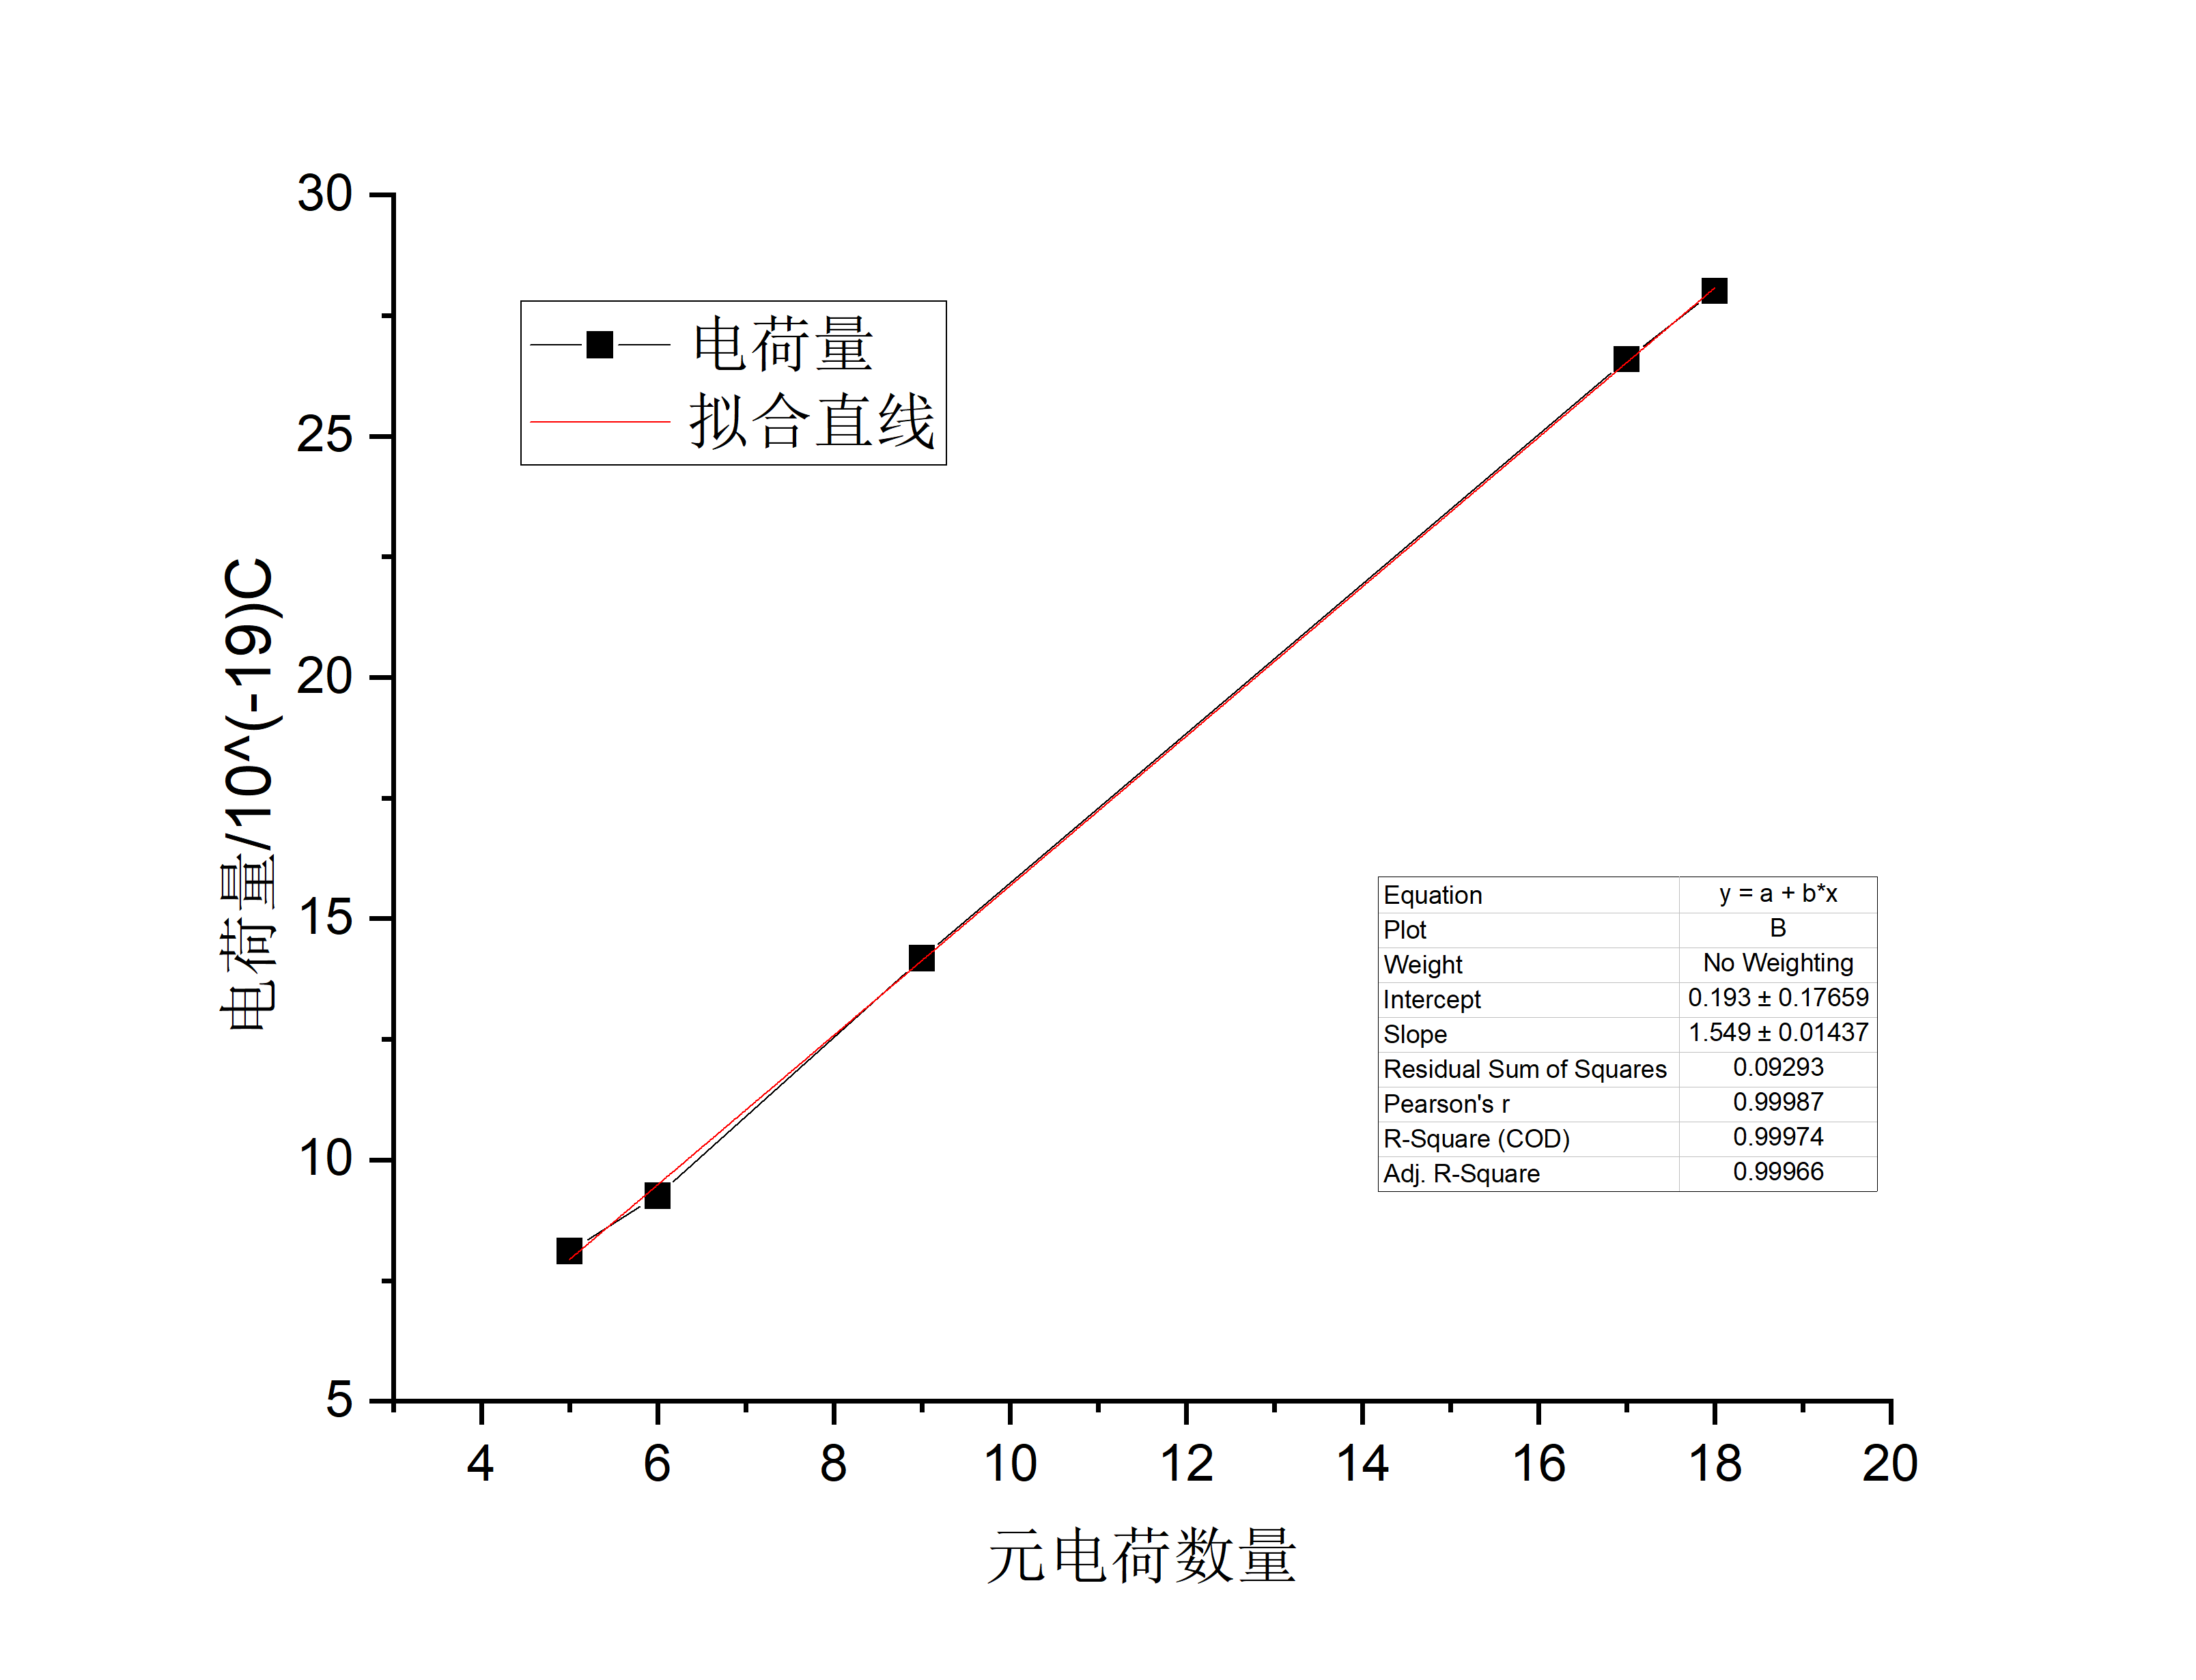
\includegraphics[width=0.6\textwidth]{img//2.png}
		%textwidth:正文宽度。双栏,则将两栏正文宽度相加。
	\caption{动态测量法的q-n拟合曲线}
	\label{fig:2}
\end{figure}

通过静态测量法实验测得的元电荷的平均值为$1.549 \times 10^{-19}C$,与标准值$e =1.602177\times 10^{-19}C$相对误差为3.31\%.

\subsubsection*{误差分析}
动态法产生误差的原因可能有:
\begin{enumerate}
	\item 油滴通过计时起点和计时终点时只有一瞬间,人的反应时间会造成时间测量的误差
	\item 油滴经过开始计时刻度线时还未到达匀速的状态,在计时的运动过程 中并非全过程匀速运动,从而造成误差
\end{enumerate}

动态法相对静态法误差较大,静态法各组数据更接近理论值,基本验证了电荷的不连续性,测出元电荷e的大小。

\subsection*{3.大量油滴带电量分析}

将所测10 个油滴带电量随元电荷个数曲线拟合得图\ref*{fig:3}:

\begin{figure}[!h]
	\centering
	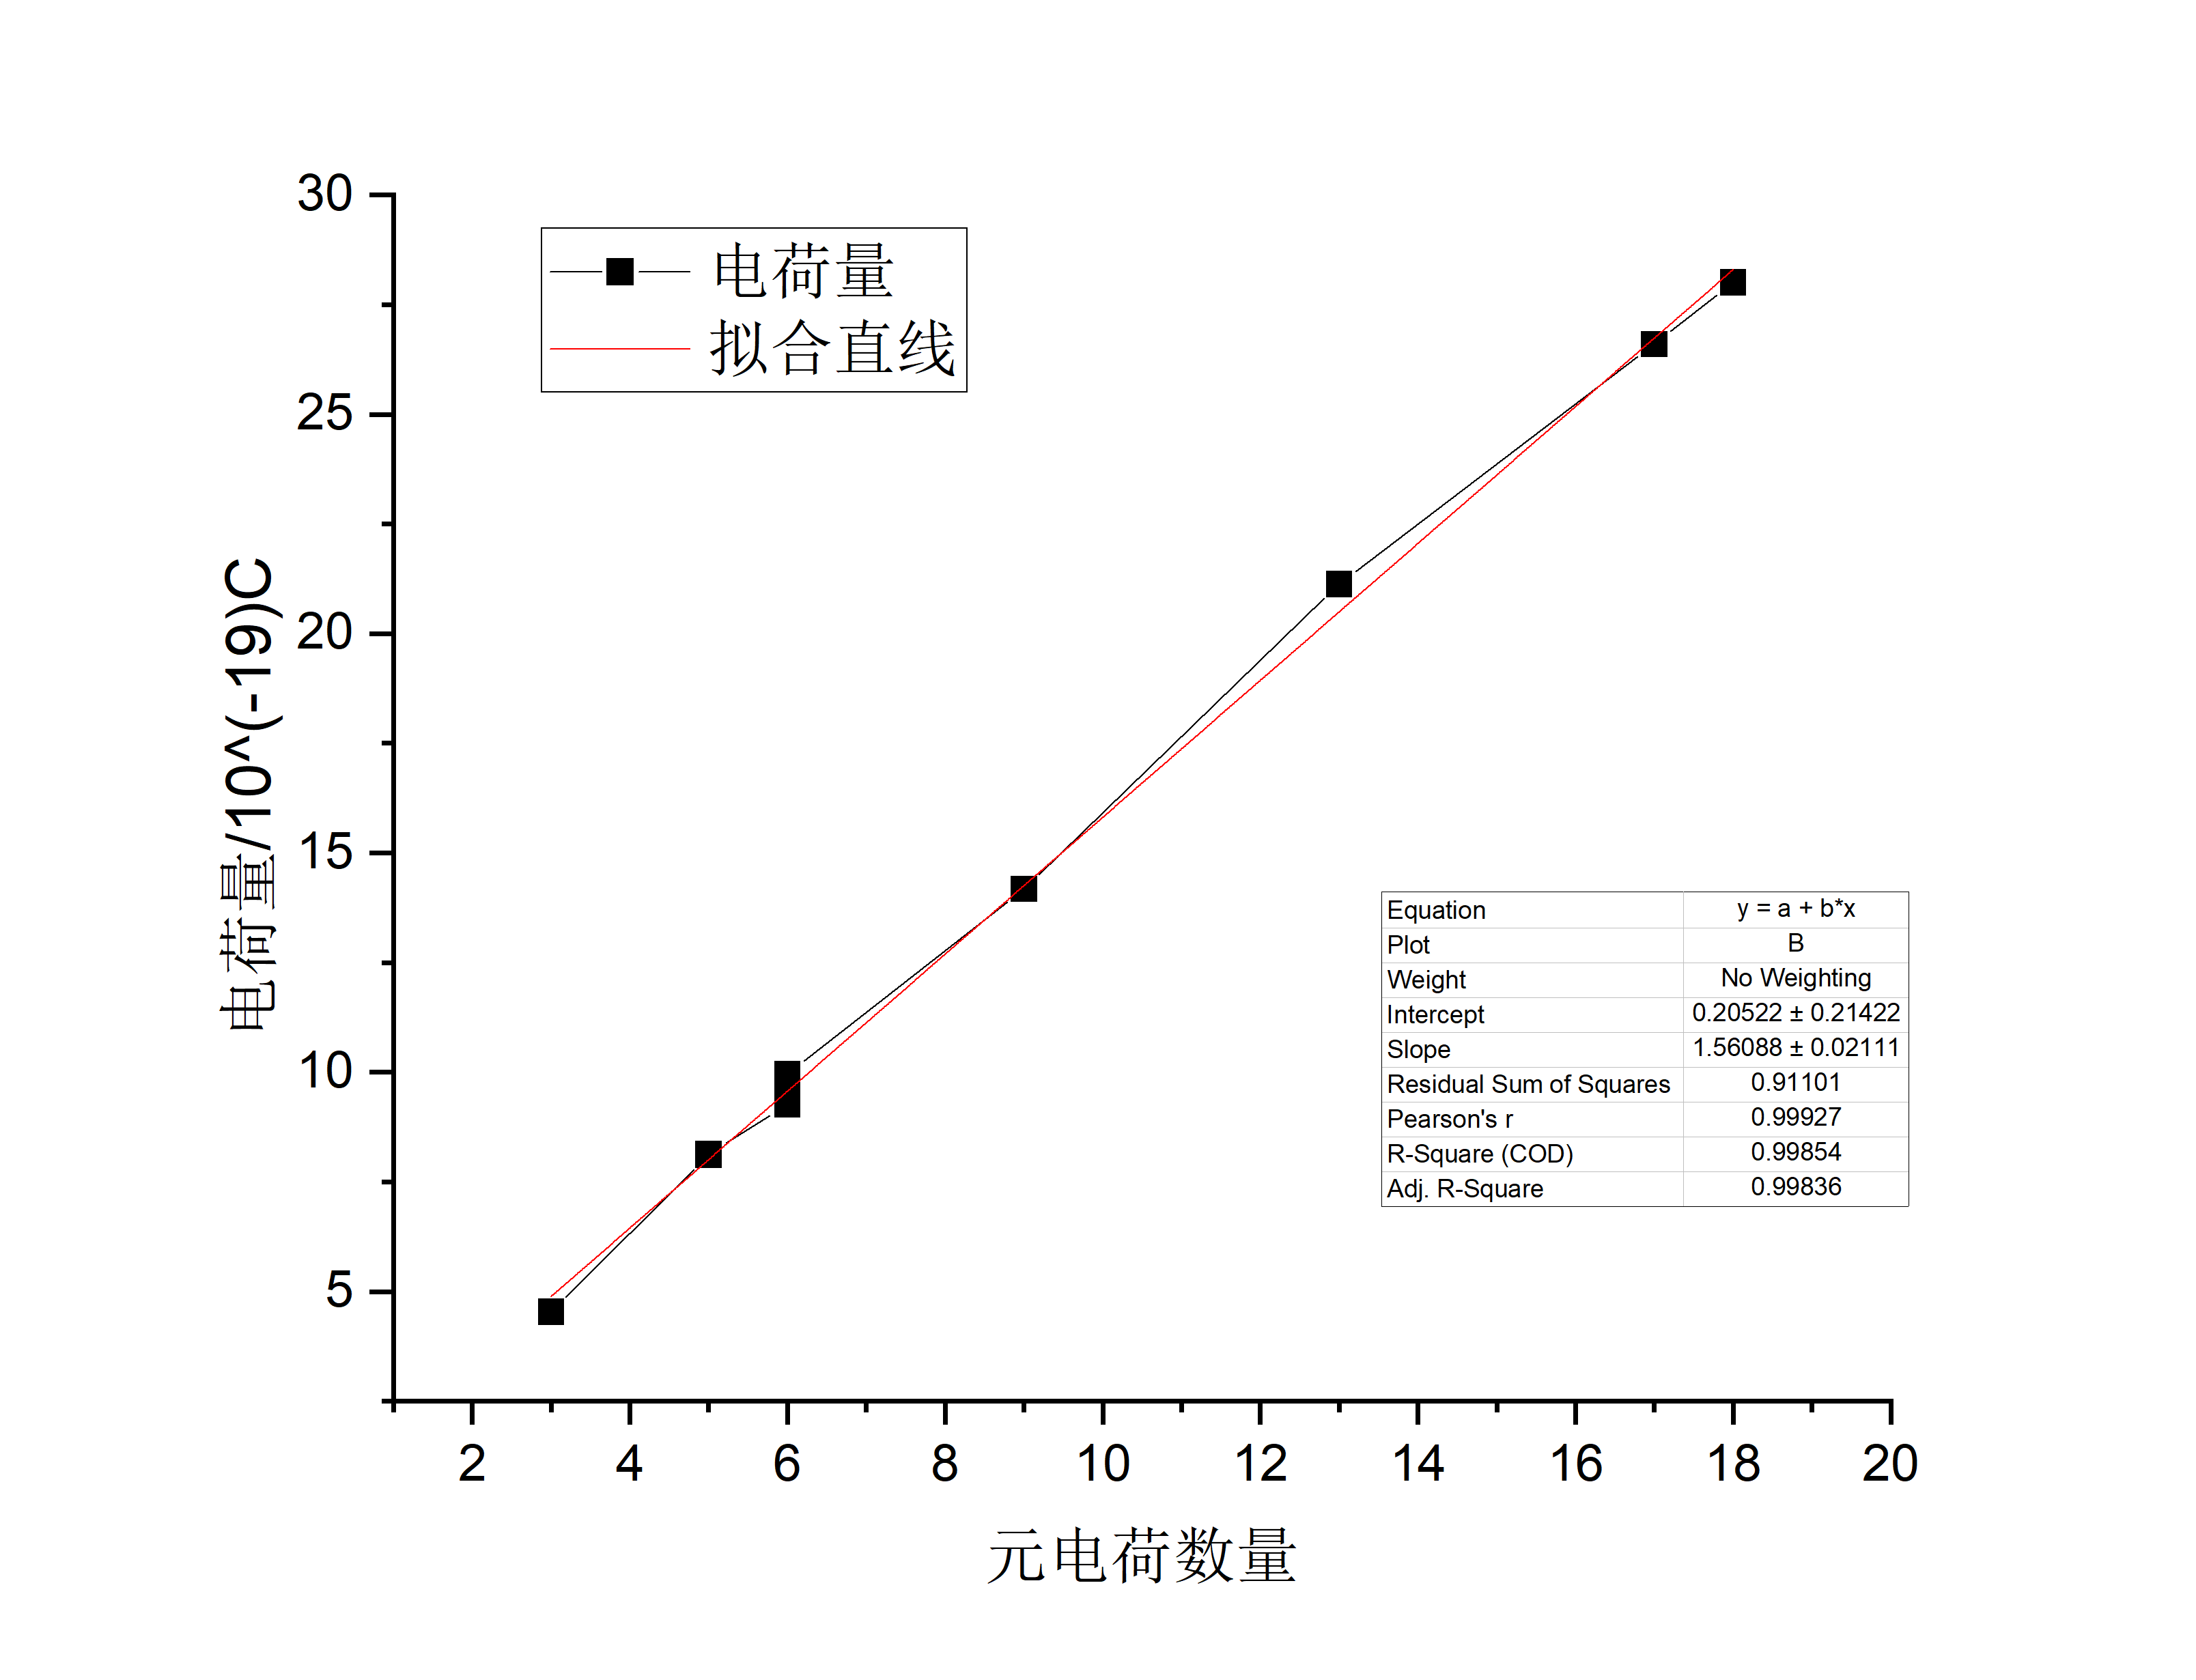
\includegraphics[width=0.6\textwidth]{img//3.png}
		%textwidth:正文宽度。双栏,则将两栏正文宽度相加。
	\caption{大量油滴q-n拟合曲线}
	\label{fig:3}
\end{figure}

通过动态测量法实验测得的元电荷的平均值为$1.56088 \times 10^{-19}C$,与标准值$e =1.602177\times 10^{-19}C$相对误差为2.58\%.

\subsubsection*{误差分析}
误差的原因可能有:
\begin{enumerate}
	\item 用于分析的数据量不够多,拟合效果不佳,误差较大
\end{enumerate}

\section*{【参考文献】}
\begin{enumerate}
	\item 沈韩.基础物理实验[M].科学出版社,2015.
\end{enumerate}

\newpage
\section*{【思考题】}
\subsection*{1.本实验如何通过宏观量测量围观量?}
答:本实验通过分析大量的宏观测量数据,得到微观量的统计规律。
通过带电油滴在重力场和电场作用下的平衡运动来建立宏观量和微观量之间的联系,
油滴的运动是可观测的,其重力(质量)也是可以在宏观的尺度下测得的,外加电场可直接通过仪器读数,有了这些表达量就可以测量微观的电荷。
\subsection*{2.实验中如何保持油滴匀速运动?}
答:实验时在视野范围内尽可能让油滴开始运动的位置离计时开始的刻度线远一些。
让油滴在距计时开始刻度线前一段距离开始加速运动。一定速度后,油滴受到的空气阻力与重力平衡,保证油滴在到达刻度线时的速度已达到最终匀速运动的速度。

\end{document}
